\chapter{Facility Layer \label{chap:facilitylayer}}
\section{Komponenten}
\begin{figure}[htbp]
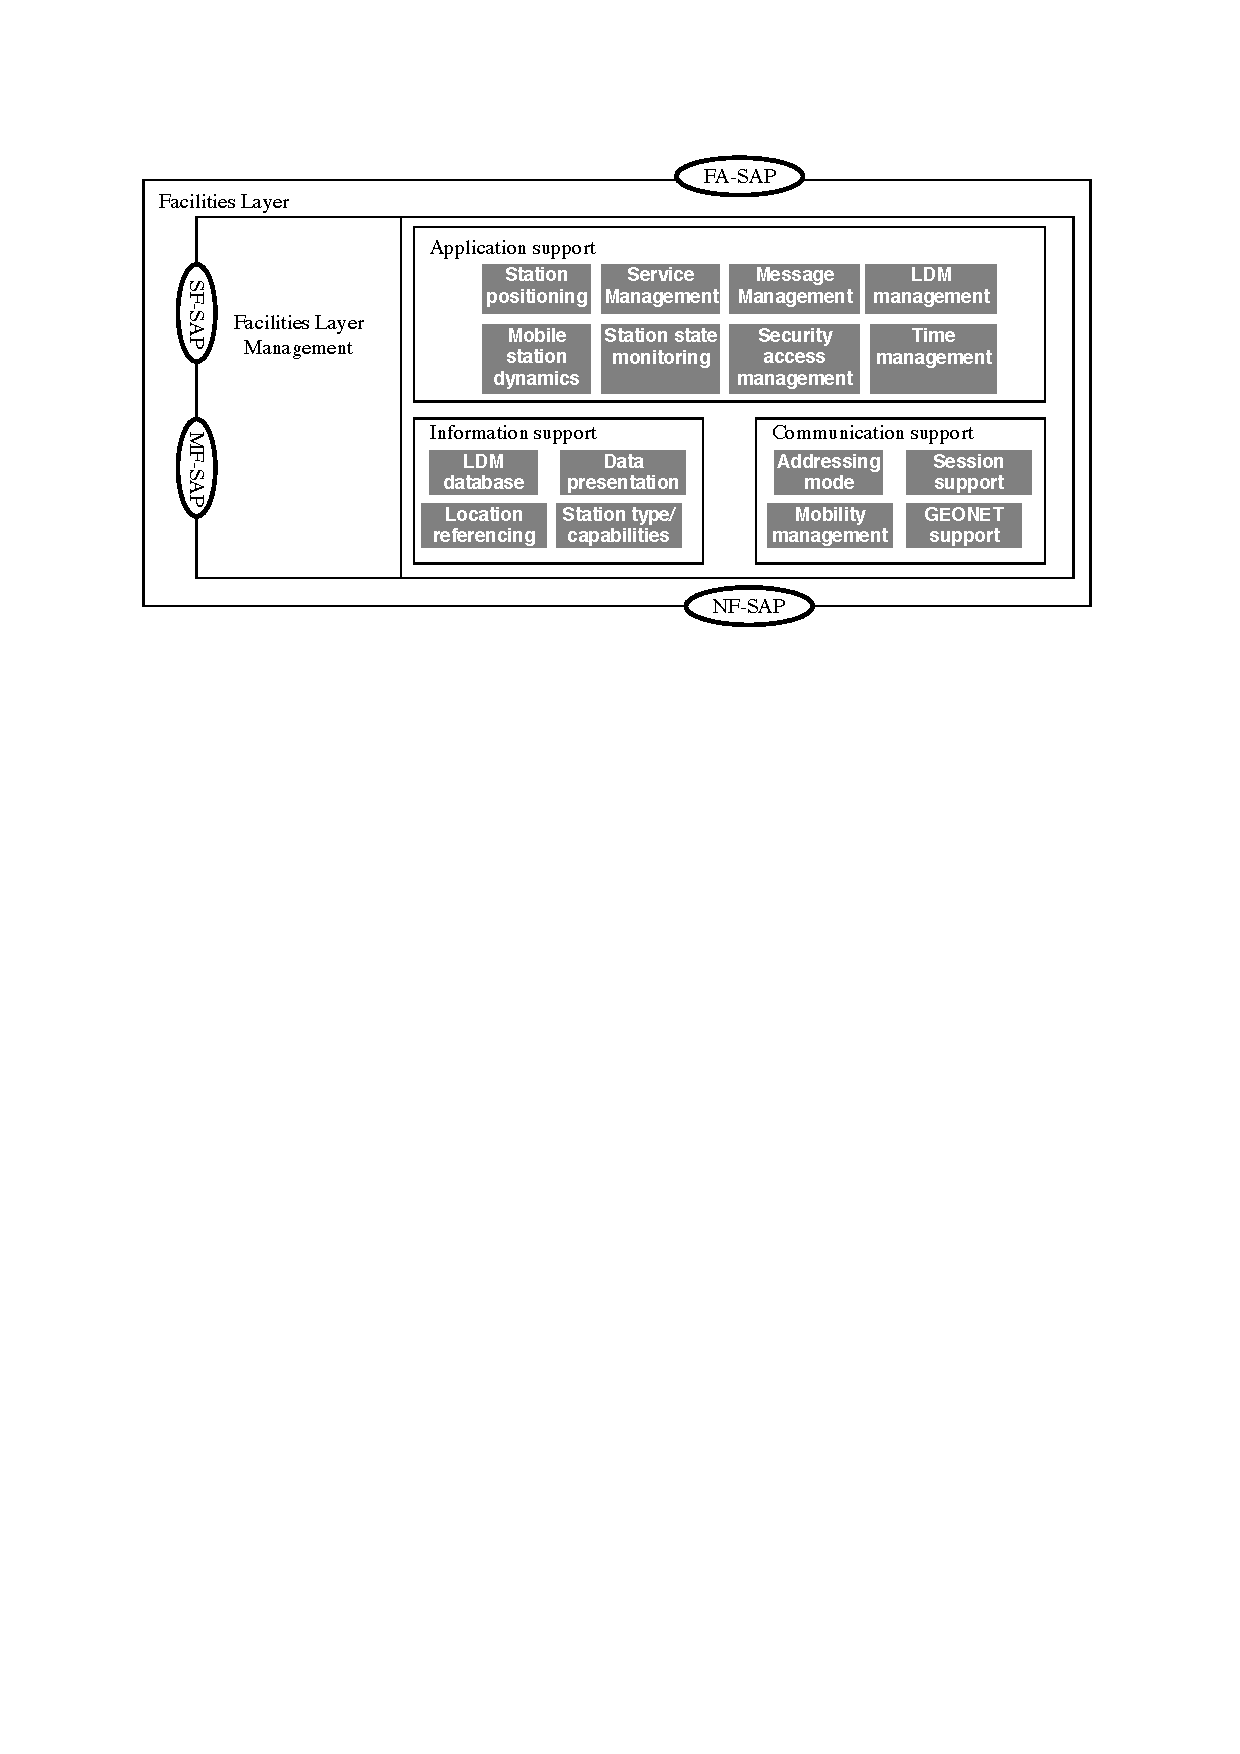
\includegraphics[width=0.99\textwidth]{content/images/04_facilitylayer/facility_layer_model.pdf}
\caption{Die Komponenten der \acl{C2C}}
\label{fig:komponentenfacility}
\end{figure}
Der Facility Layer liegt unterhalb des Applicationlayer und teilt sich in drei Hauptkomponenten auf. Er bietet verschiedene allgemeine Services an die von den Anwendungen des Application Layer verwendet werden können.

\subsection{Application Support}
Der Application Support stellt die Grundfunktionalität für die Anwendungen zur verfügung. Darunter fällt das station lifecycle management, das automatische erkennen von Services sowie das downloaden und initialisieren von neuen Services und noch weitere. Die einzelne Komponenten des Application Support, die auf der \autoref{fig:komponentenfacility} zu sehen sind, werden im folgenden genauer erläutert. 

\subsubsection{Station positioning}
Dieser teil des Application Support verarbeitet die Informationen die aus den verschiedenen Datensammler gewonnen werden wie aus GNSS oder aus Fahrzeugsensoren um die Position des Station zu gewinnen. 
Da diese Angaben sehr genau sein müssen werden die Daten in 3D Position gemessen (latitude, longitude, altitude). Dies können, durch beispielsweise GPS, in Echtzeit zur verfügung stehen. Da es jdeoch Sicherheitsbedingte Anwendungen gibt bei denen bereits über 0.5m Abweichung eine fatale Auswirkung haben kann, werden die Standortinformationen noch einmal über weitere Einheiten verbessert. Dazu gehören z.b. Odometer oder Gyroskop.
Damit diese Support facility ihren Aufgaben Nachkommen kann, ist im \cite{etsi102638} folgende Vorraussetzungen definiert.

\begin{itemize}
\item Benötigt Verbindung zwischen ITS station und einem GNSS system. Bei kurzfristigen Ausfall der Verbindung übernehmen interne mechanische Fahrzeugsensoren wie das Gyroskop oder das Odometer.
\item Benötigt dauerhafte Verbindung zu den Fahrzeugsensoren (direkte Verbindung oder über einen Bus).
\item Benötigt genug Rechenleistung um 3D Positions Angaben sicher zu Verwalten und zu Berechnen.
\end{itemize}

\subsubsection{Mobile station dynamic monitoring}
Das Mobile station dynamic monitoring ist nur für die \acs{VS} verfügbar. Diese Einheit des Facility Layer verwaltet eine große Anzahl an Fahrzeugspezifischen Daten die von den Applicationen und anderen Komponenten des Facility Layers verwendet werden. Sie ist dafür verantwortlich diese Daten immer auf dem neueste  Stand zu halten. 

\begin{itemize}
\item Benötigt zugriff auf Fahrzeug Funktionen wie das Bremssystem, Reifendruck, Stabilitätskontrolle, Geschwindigkeitsregelung etc.
\item Benötigt 
\item Benötigt genug Rechenleistung um 3D Positions Angaben sicher zu Verwalten und zu Berechnen.
\end{itemize}Diese Einheit benötigt die folgenden Vorraussetzungen.



This support facility requires access to vehicle functions according to selected options (e.g. braking system,
steering system, tyre pressure monitoring system, stability control system, speed control, etc.).
• This support facility requires capabilities to filter the selected parameters being needed by applications and
other facilities (e.g. master cylinder pressure, steering wheel angle, steering wheel angle rate of change,
programmed speed control value, stability control status, yaw rate, vehicle speed, acceleration control, etc.).
• This support facility requires capabilities to update parameters values being used for CAM. 


\subsubsection{Station state monitoring}

\subsubsection{Services management }

\subsubsection{LDM management }

\subsubsection{Messages management}

\subsubsection{Security access management}
\subsubsection{Time management}
\subsubsection{Time management}
\subsubsection{Time management}

\subsection{Information Support}
The information support covers the presentation layer of the OSI reference model and holds the role of
data management. In any ITS system, there will be an abundance of data sources, both mobile and static
ones. These data will mostly be location referenced, time specific and attached with life time value and
with accuracy and reliability parameters. Therefore, fusing data and keeping the information up to date is
one of the challenges of information support. Main entity that supports this is Local Dynamic
Map (LDM) that is able to take data both from different sources and from received ITS messages to build
a data model of the local environment. Furthermore, the information support takes on many functions of
the OSI Presentation Layer. 
\subsubsection{LDM database}
\subsubsection{Data presentation}
\subsubsection{Location referecing}
\subsubsection{Station type/capabilities}

\subsection{Communication Support}
The communication support, which includes the session layer of the OSI Reference model. It will
cooperate with the transport and network layer to achieve the various communication modes required by
the applications. 

\section{CAM\label{sec:cam}}

\section{DEN\label{sec:den}}


\section{SPaT\label{sec:spat}}
\ac{SPaT} ist eine Nachricht, die den Zustand einer Straßenkreuzung beschreibt. Die Beschreibung enthält Staus Informationen der \ac{VBA}. Diese enthalten allgemeine Betriebszustände,  

Für \ac{SPaT} gibt es zwei grundsätzliche Betriebsarten. Die erste Betriebsart ist eine feste \ac{VBA} Schaltung. Diese wird den \ac{IVS} über \ac{SPaT} Nachrichten mitgeteilt. Anhand dieser Informationen kann das \ac{IVS} selber die Ampelzeiten berechnen und benötigt keine  weiteren \ac{SPaT} Nachrichten. Die zweite Betriebsart ist, dass die Ampelzeiten aufgrund externer Ereignisse beeinflusst werden können. Externe Ereignisse sind beispielsweise Fußgänger, verkehrsabhängige Schaltungen oder periodisierte \ac{IVS}, wie z.B. Rettungswagen. Bei der zweiten Betriebsart muss beachtet werden, dass zu schnelle Änderungen vermieden werden müssen. Die \ac{IVS} benötigen eine bestimmte Zeit zur Reaktion, so benötigt beispielsweise ein Auto die Reaktionszeit des Fahrers und einen Bremsweg. Wird die Fahrspur dieses Autos gesperrt und andere Fahrspuren dafür freigegeben, wenn das Auto sich schon fast vor der Haltelinie befindet, so ist eine Bremsung vor der Kreuzung nicht mehr möglich. Daraus resultiert ein Sicherheitsrisiko, da die andere Fahrspur nicht für die anderen Fahrzeuge garantiert frei ist. \todo{Rausfinden, ob die \ac{IRS} die Position des \ac{IVS} verwertet und daraus die Zeiten generiert. S.29 US Department.. -> Ich glaube die verwendet die Daten}

Auf dieser Grundlage können weitere Dienste angeboten werden. So können Abbiegeassistent Systeme oder Vorzugsschaltungen realisiert werden. 

 Abbiegeassistent Systeme unterstützen \ac{IVS} beim Abbiegen in Kreuzungen. Anhand der Positions- und Geschwindigkeitsdaten der \ac{IVS} kann die \ac{IRS} berechnen, ob ein Abbiegen nach rechts oder nach links sicher ist. Neben der Positionsdaten können auch Erfassungssysteme genutzt werden, die in die Infrastruktur integriert sind. Beispiele hierfür können \ac{Radar} oder \ac{Lidar} Systeme genutzt werden. Der Nachteil von rein \ac{ITS} basierten Systemen ist, dass nicht \ac{ITS} kompatible Fahrzeuge nicht erkannt werden. Das bedeutet, dass die \ac{IRS} eine freie Kreuzung erkennt und meldet, obwohl nicht \ac{ITS} basierende Fahrzeuge über die Kreuzung fahren. 
 
Die Bevorzugung von Fahrzeugen bietet sich für die Empfehlung \cite{usSpat} für Notfallfahrzeuge, für Fahrzeuge des Nahverkehrs und für den Frachtverkehr an. Durch die Bevorzugung können diese \ac{IVS} eine grüne Welle erreichen. Das bedeutet, dass entweder Grünphasen verlängert werden oder Rotphasen unterbrochen werden. Sofern nicht bereits durch andere Nachrichten, wie \ac{CAM} geschehen, fordert das \ac{IVS} bei der \ac{IRS} eine Bevorrangung an, wenn anhand der \ac{SPaT} erkennt, dass die Kreuzung nicht frei ist. Die \ac{IVS} beantwortet diese Anfrage im positiven Fall mit einer weiteren \ac{SPaT} Nachricht, die eine freie Kreuzung signalisiert.   

Inhalt einer \ac{SPaT}:
\begin{longtable}{|c|c|}
 \hline
Datenelemente & Typ/Größe\\
 \hline
Object ID & Unsigned 8 Bit Integer\\
 \hline
 Object Size& Unsigned 8 Bit Integer\\
 \hline
 Apptoach ID& Unsigned 8 Bit Integer\\
 \hline
 Signal Phase Indication &  32 Bit Bitmask \\
 \hline
 Countdown Timer Confidence & 32 Bit Bitmask \\
 \hline
 Time to Signal Phase Change (Countdown Time) & Unsigned 16 Bit Integer \\
 \hline
 Yellow Duration & Unsigned 8 Bit Integer\\
 \hline
 \caption{Inhalt einer SPaT Nachricht \cite{usSpat}}
 \label{tab:facilitylayer_inhaltSpatNachricht}
 \end{longtable}

\section{TOPO\label{sec:topo}}
